\subsection{오류 유형 및 사례 분석}

\label{sec:ch4_5}

4.2–4.4의 평균 차이를 문항 수준 변화로 보이기 위해, 문항별 gold 출현 443건(집계 방식은 S4)을 최초 탈락 단계 또는 최종 선택 상태에 배정하였다(그림~\ref{fig:ch4_5}). corpus 미매핑과 BM25 미회수는 두 조건에 공통이었고, shortlist 탈락은 CE 42건에서 Jev 13건으로 줄었으나 shortlist에 남은 뒤 미선택된 출현은 60건에서 72건으로 늘었다.

\begin{figure}[H]
\centering
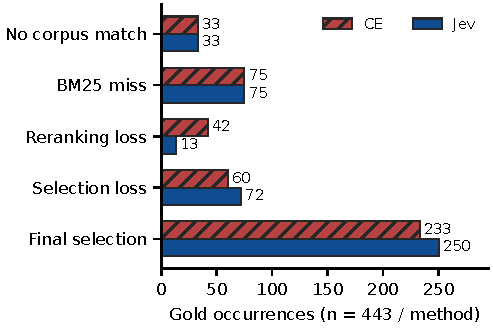
\includegraphics[width=\linewidth]{research/chapter4/figures/section-figures-v1/fig_4_5_gold_loss_stages_column.pdf}
\caption{문항별 gold 출현 443건의 배타적 단계 분류. Reranking loss는 shortlist 탈락, Selection loss는 미선택이며, 미선택은 목록별 선택 수 제약의 영향도 받는다.}
\label{fig:ch4_5}
\end{figure}

개선·CE 우세·지표 불일치 집단에서 F1 차이 절댓값이 집단 중앙값에 가장 가까운 문항을 대표 사례로 선정하였다(식별자·선정 규칙·원문 위치는 S4). 식품 생산실적과 회수계획의 보고 상대방을 묻는 개선 사례에서 Jev는 식품위생법 제42조제2항을 유지하면서 제45조제1항을 추가로 확보하여, 근거 F1이 50$\to$100, LF-Eval이 65.29$\to$99.18로 높아졌다. 복수 당사자 청구 절차 사례에서는 gold인 민사소송법 제79조제1항이 Jev의 shortlist에서 탈락하고 제83조제1항이 선택되어, F1은 80$\to$40, LF-Eval은 71.79$\to$52.67로 낮아졌다. 사면과 복수 범죄 처리 사례는 gold 3개에 후보 목록이 2개뿐이었고(하나는 corpus 미매핑, 하나는 BM25 미회수), Jev는 CE가 선택한 나머지 gold도 확보하지 못해 근거 F1이 40$\to$0으로 낮아졌지만 Token F1은 18.60$\to$25.88로 상승하였다. 사례 분석은 자동 관측에 근거하며 정답 외 조문의 법률적 적절성은 판정하지 않았다.

종합하면, 저장된 단일 Jev 실행에서 재정렬기 교체는 shortlist의 gold 유지를 늘렸고(RQ2), 이와 함께 평균 근거 F1이 3.19점 높아졌으나 EM·완전 회수 차이는 불확실했으며 차이는 주로 2·3-hop 문항에서 관측되었다(RQ1). 자동 답변 지표도 소폭 높아졌으나 Token F1의 개선은 경계적이었고 입력량 절감은 관찰되지 않았다(RQ3). 재정렬 단계 지연은 약 2.25배 길었으나 배포 조건에 의존하며 품질(226문항)과 다른 실행·표본(60문항)에서 측정되었다. 공개 코드의 후보 목록 참조 수정에 따른 F1 차이(9.85점)는 재정렬기 교체에 따른 차이보다 컸다.
